
\PassOptionsToPackage{table}{xcolor}

\documentclass[]{lsstbeamer}

\usepackage{animate}
\usepackage{media9}
\usepackage{times,amsmath,graphicx,marvosym}
\usepackage{multirow,array,colortbl,multimedia}

\usepackage{tikz,multirow,array,colortbl,multimedia}
\usetikzlibrary{arrows,shapes,decorations.shapes,shadows,calc}
\usetikzlibrary{shapes.callouts, decorations.text}
\usetikzlibrary{calc}

\tikzstyle{flow}=[->, >=stealth', thick, shorten >=3pt, shorten <=3pt]



\usepackage{pgf}

% ----------------------
%
%\setLogoleft{\colorbox{white}{\includegraphics[height=1.5cm]{images/logoDG}}}

%\logoleft{GaiaTrans}


\author[William O'Mullane]{William O'Mullane }

\date[05/03/2017]{ 5$^{\text{th}}$ March  2017, LSST JTM, \\ LA, California, USA. }


\institute[LSST]{Data Management\\LSST}
% ----------------------


\AtBeginSection[]  % "Beamer, do the following at the start of every section"
{
\begin{frame}<beamer>
\addtocounter{framenumber}{-1}
\frametitle{Outline} % make a frame titled "Outline"
\tableofcontents[currentsection]  % show TOC and highlight current section
\end{frame}
}


\AtBeginSubsection[]
{
   \begin{frame}
\addtocounter{framenumber}{-1}
       \frametitle{Outline}
       \tableofcontents[currentsection,currentsubsection]
   \end{frame}
}


%
% Empty frame environment: useful for page-filling images.
%
% argument is frame title
%
\newenvironment{emptyframe}[1]{%
\begin{frame}[plain]
  \hypertarget<1>{#1}{}
  \only<1>{\pdfbookmark[2]{#1}{#1}}}%
{\end{frame}}




\title[DM Organisation]{DM organisation and reviews  }




% ----------------------


\AtBeginSection[]  % "Beamer, do the following at the start of every section"
{
\hspace*{10pt}
\begin{frame}<beamer>
\frametitle{Outline of the talk } % make a frame titled "Outline"
\tableofcontents[currentsection]  % show TOC and highlight current section
\end{frame}
}


\begin{document}

\frame[plain]{\titlepage }
\section{Introducion}


\frame{\frametitle{ A little about myself}
\begin{itemize}
\item 1985ish Life started with BASIC on a  commodore 
\item 1993 graduated  Computer Science Degree and Masters University College Cork, Ireland 
\item 1993 - 1997 Spacecraft Control Systems (C++) in ESA Mission Operations Centre Darmstadt Germany
\item 1997 - 2001 Hipparcos, Integral, Planck, Gaia, Bepi-Sax  (C,Java,Oracle, HTM, HEALPix) in ESA Technology Research Centre Noordwijk Netherlands
\item 2001-2003 Commercial programming - some Astronomy (Java) 
\item 2003-2005 The Johns Hopkins, SDSS and National Virtual Observatory (C,C\#,Java,Sqlserver)
\item 2005-2014 Gaia Astrometric Solution and Science Operations (Java, Oracle, Intersystems Cache) 
\item 2012  PhD in Physics on Implementing the Gaia Astrometric Solution,  Barcelona University
\item 2014-2017 All ESA Science Ground Segments in Development
\end{itemize}
}

\frame{\frametitle{Induction to astronomy : HIP Catalogue}
1997/98 Hipparcos Java Tools - learning Astrometry
\url{http://www.cosmos.esa.int/web/hipparcos/java-tools}
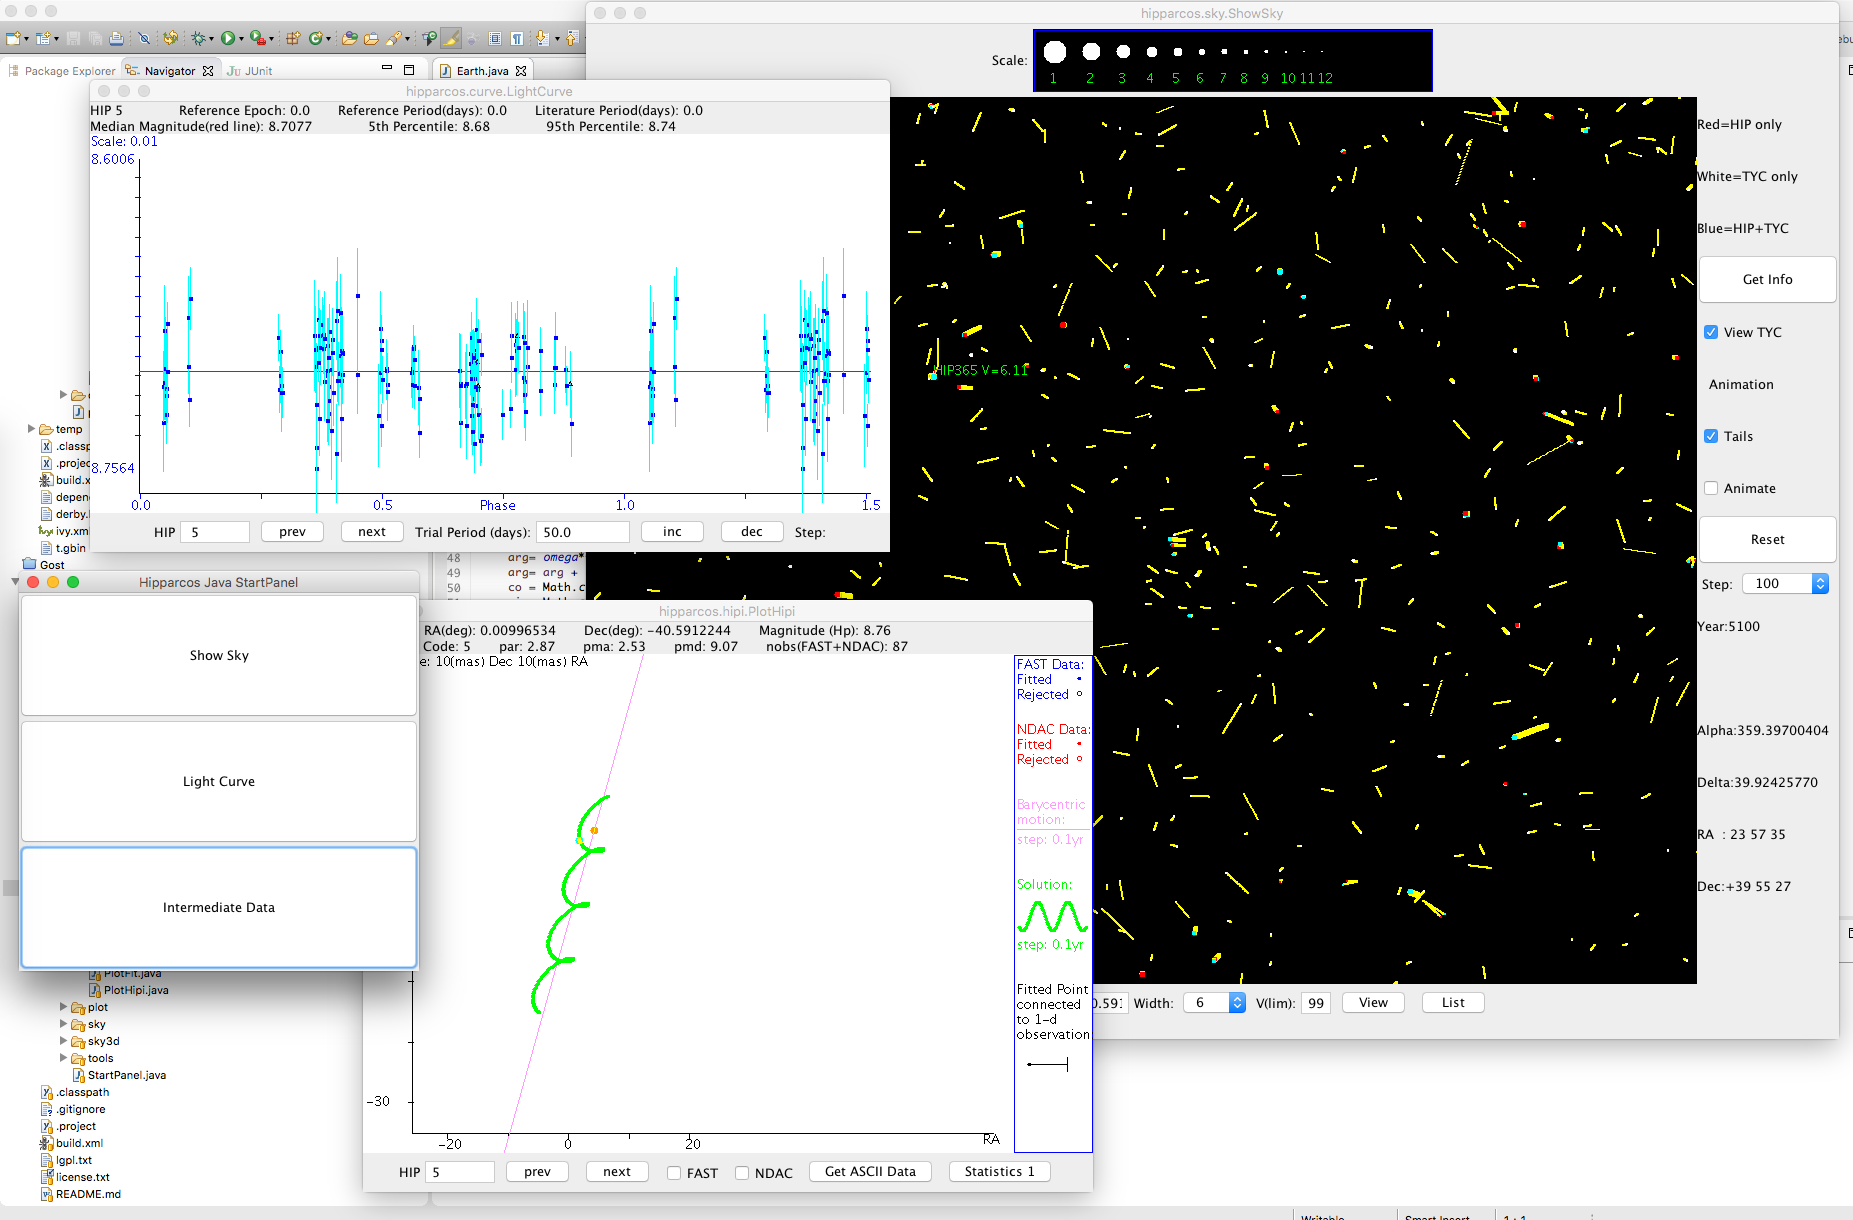
\includegraphics[width=\textwidth]{hipjt}
}

\frame{\frametitle{In the USA .. }
\vspace{5pt}
\begin{columns}[c]
\column{0.6\textwidth}
\vspace{4pt}
Quality tools for GSC2 (Java) $\rightarrow$\\
\vspace{8pt}
CasJobs (C\#)\citep{conf:casjobs}
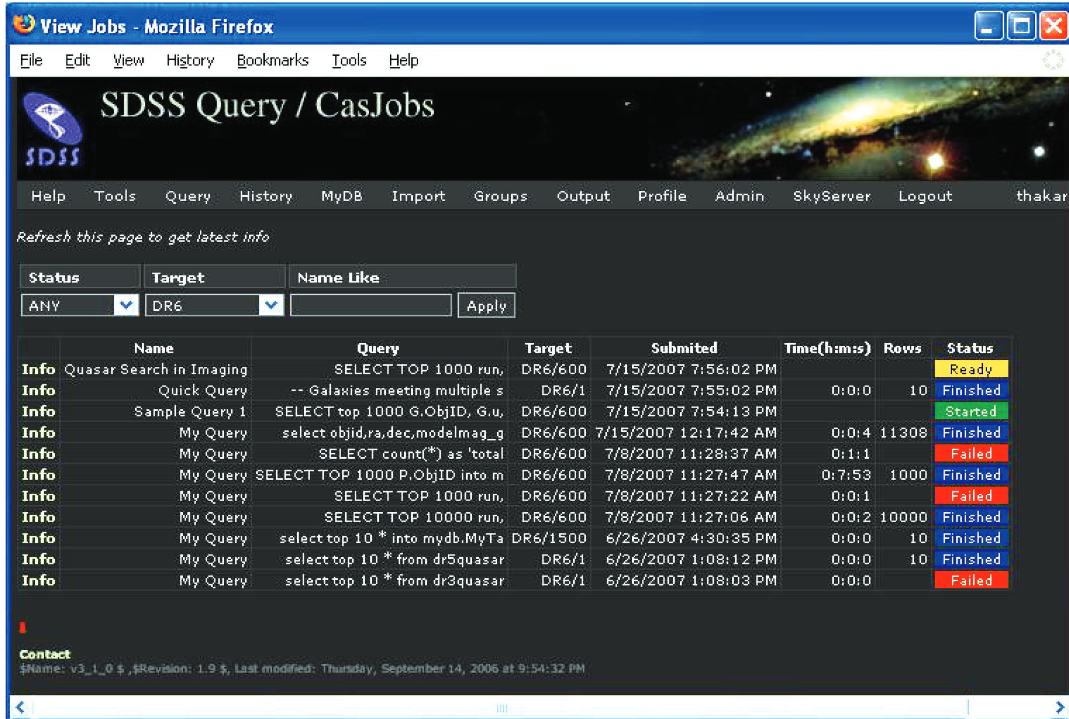
\includegraphics[width=\textwidth]{casjobs}
\column{0.4\textwidth}
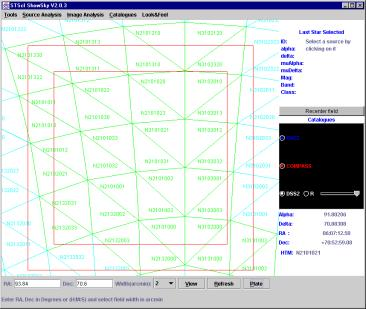
\includegraphics[width=\textwidth]{sshtm}
\vspace{-1cm}
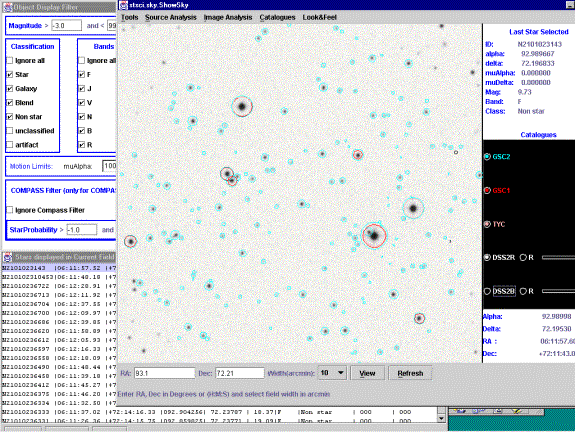
\includegraphics[width=\textwidth]{showsky}
\end{columns}
}


\frame{\frametitle{European Space Astronomy Centre }
\begin{columns}[c]
\column{0.4\textwidth}

\includegraphics[width=0.9\textwidth]{exm}\\

\includegraphics[width=0.45\textwidth]{bepiclogo}
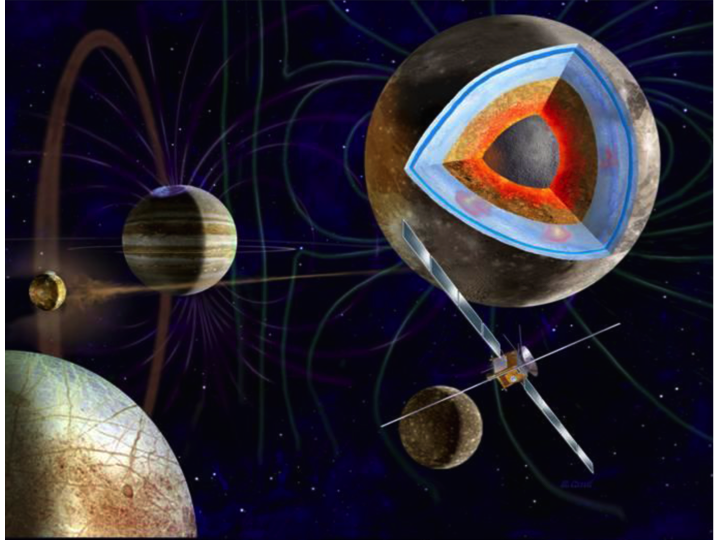
\includegraphics[width=0.45\textwidth]{juice}\\
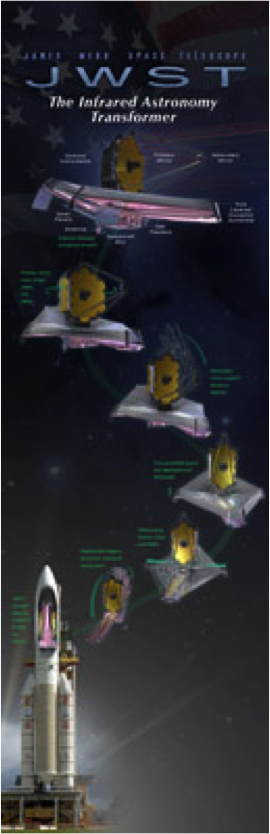
\includegraphics[width=0.45\textwidth]{jwst}\\
\vspace{-6cm}
\hspace{2.2cm}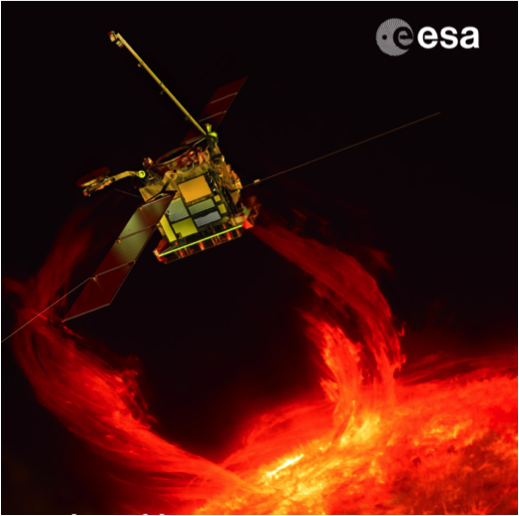
\includegraphics[width=0.45\textwidth]{solo}\\
\hspace{2.2cm}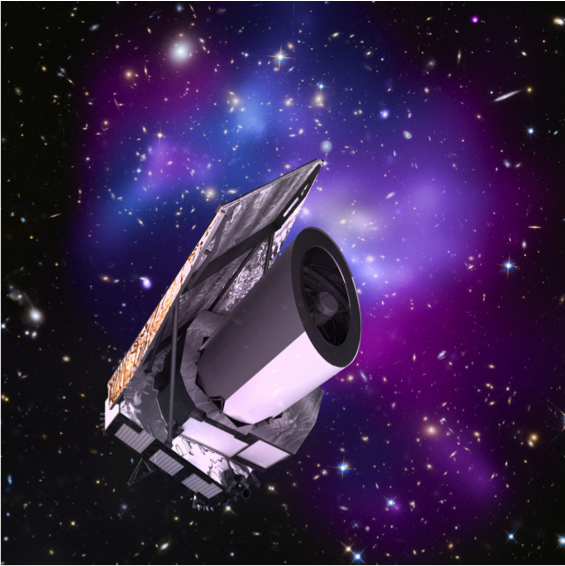
\includegraphics[width=0.45\textwidth]{euclid}

\column{0.6\textwidth}
\begin{itemize}
\item ESAC Located near Madrid, Spain.
\item Home of the Science Operations Department  containing  Operations Development Division.
\item Develop Science Operations Systems:
\begin{itemize}
\item People, Procedures and Software.
\item Interactions MOC and scientific communities.
\item Quite a bit of software - diverse - mainly Java but FORTRAN, C, C++, Python ..
\item Prepare for planning, simulations, instrument performance, commanding.
\item Hand over system to operations division after commissioning.

\end{itemize}
\end{itemize}
\end{columns}
}




\section{DM Organisation }
\frame {\frametitle{ Data management }
    \begin{itemize}
	\item Victor remains interim PM until April 
	\item Have been trying to get an idea of DM organisation - talking to DMLT and TCAMS 
	\item Following are some observations and draft ideas 

    \end{itemize}

    {\bf   Look out for a  new version of LDM-294 - DM Management Plan}
    \begin{itemize}
	\item It will detail roles and responsibilities in DM
    \end{itemize}
    \vspace{12pt}
    DM Mission :\\
    {\em  Stand up operable, maintainable, quality services to deliver high-quality LSST data products for sciencer, all on time and within reasonable cost.}
}


\frame {\frametitle{ DM Organisation}

      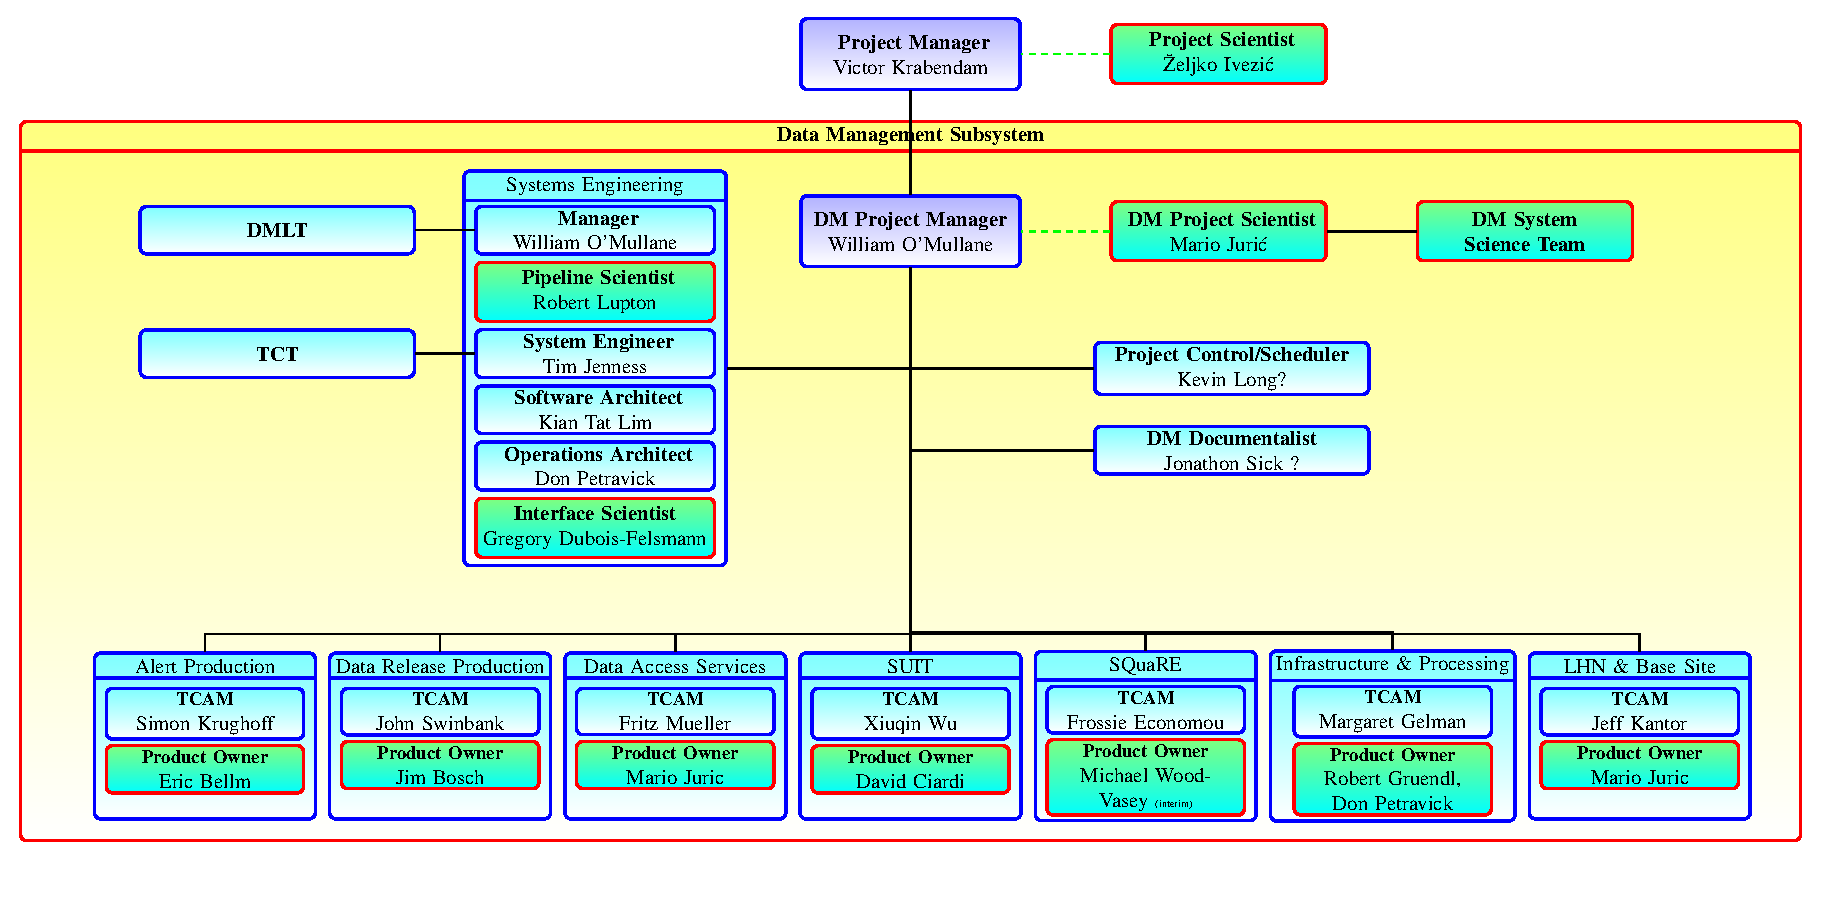
\includegraphics[width=1.0\textwidth]{images/DmOrg}\\
}

\frame {\frametitle{ DM architecture \& products}
	\begin{itemize}
	\item Would like to get  a list of products in DM
	\item Related to understanding the DM architecture - KT working on LDM-148 update more from him in a while
	\item Those are not Data Products - mostly Systems and Software artefacts
	\item For each product identify {\em Product Owner} and manager.
	\item This would change the org chart ..
	
	\end{itemize}

}

\frame {\frametitle{ Risk Management and other processes ..}
Also in LDM-294:
	\begin{itemize}
	 \item Would like an open Risk approach - anyone can raise a risk (Tim working on that)	
	 \item Document management - in next slid as
	 \item Configuration control 
	 \item Product assurance  and Scientific Validation 
	\item \ldots
	\end{itemize}
Mainly these will be high level and point to the details in other documents. 

}




\frame {
  \frametitle{  Flight Operations Procedures in MOC}
\vspace{-0.4cm}
\begin{center}
   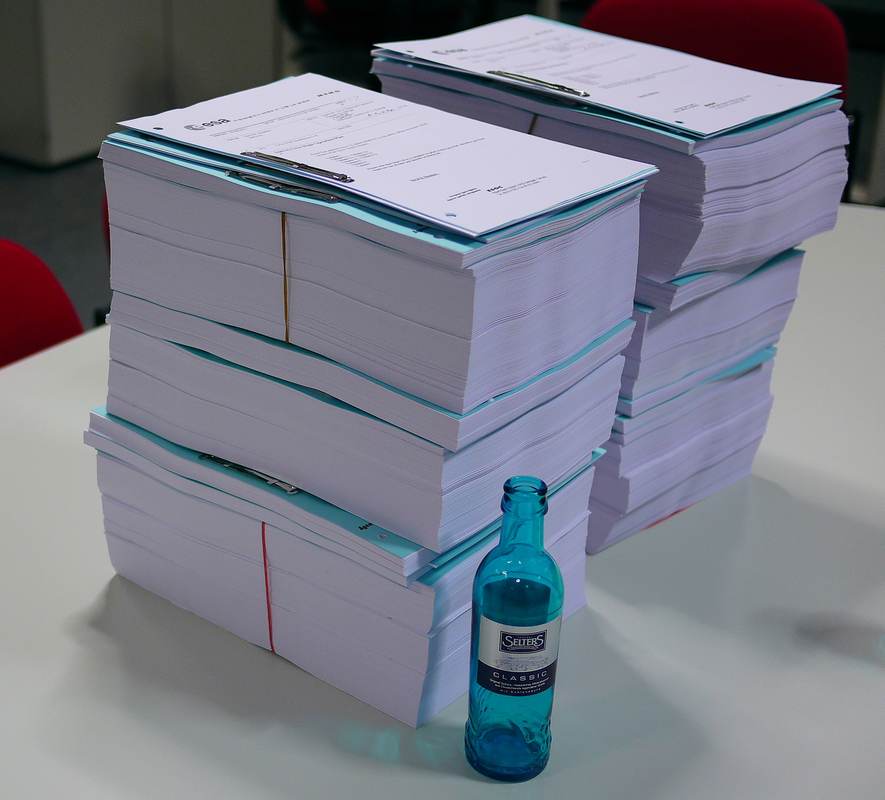
\includegraphics[width=0.6\textwidth,trim=0cm 0cm 0cm 0cm]{images/fops}\\
\end{center}
\vspace{-7pt}
The FOP is followed by the spacecraft operators - the paper copy is just in case the computers fail - could be useful!
\begin{center}
\vspace{-5pt}
{\color{red} But we should avoid {\em write only} documents.}
\end{center}
}




\frame  {\frametitle{  DM docs }

\begin{itemize}
  \item  We will be working on a Documentation Tree for DM
   \item Some documents exist - some have not yet been found
   \item Wish to figure out what is missing 
   \item LDM-294 will have a section on documentation
  \item  Adhere to LSST Document Plan LPM-051\citell{LPM-051} 
   \item Would like a bibtex file of all Docushare issued documents 

\item {\color{red} All products should be listed and for each product the set of docs expected and the dates}  
        \begin{itemize}
	\item each document type is  targeted at a different audience (e.g. Requirement, Design/Implementation, Installation, User \ldots 
	\item not all products have all document types. 
        \end{itemize}
\end{itemize}
 
}


\frame  {\frametitle{  Draft Doc Tree }
\begin{center}
 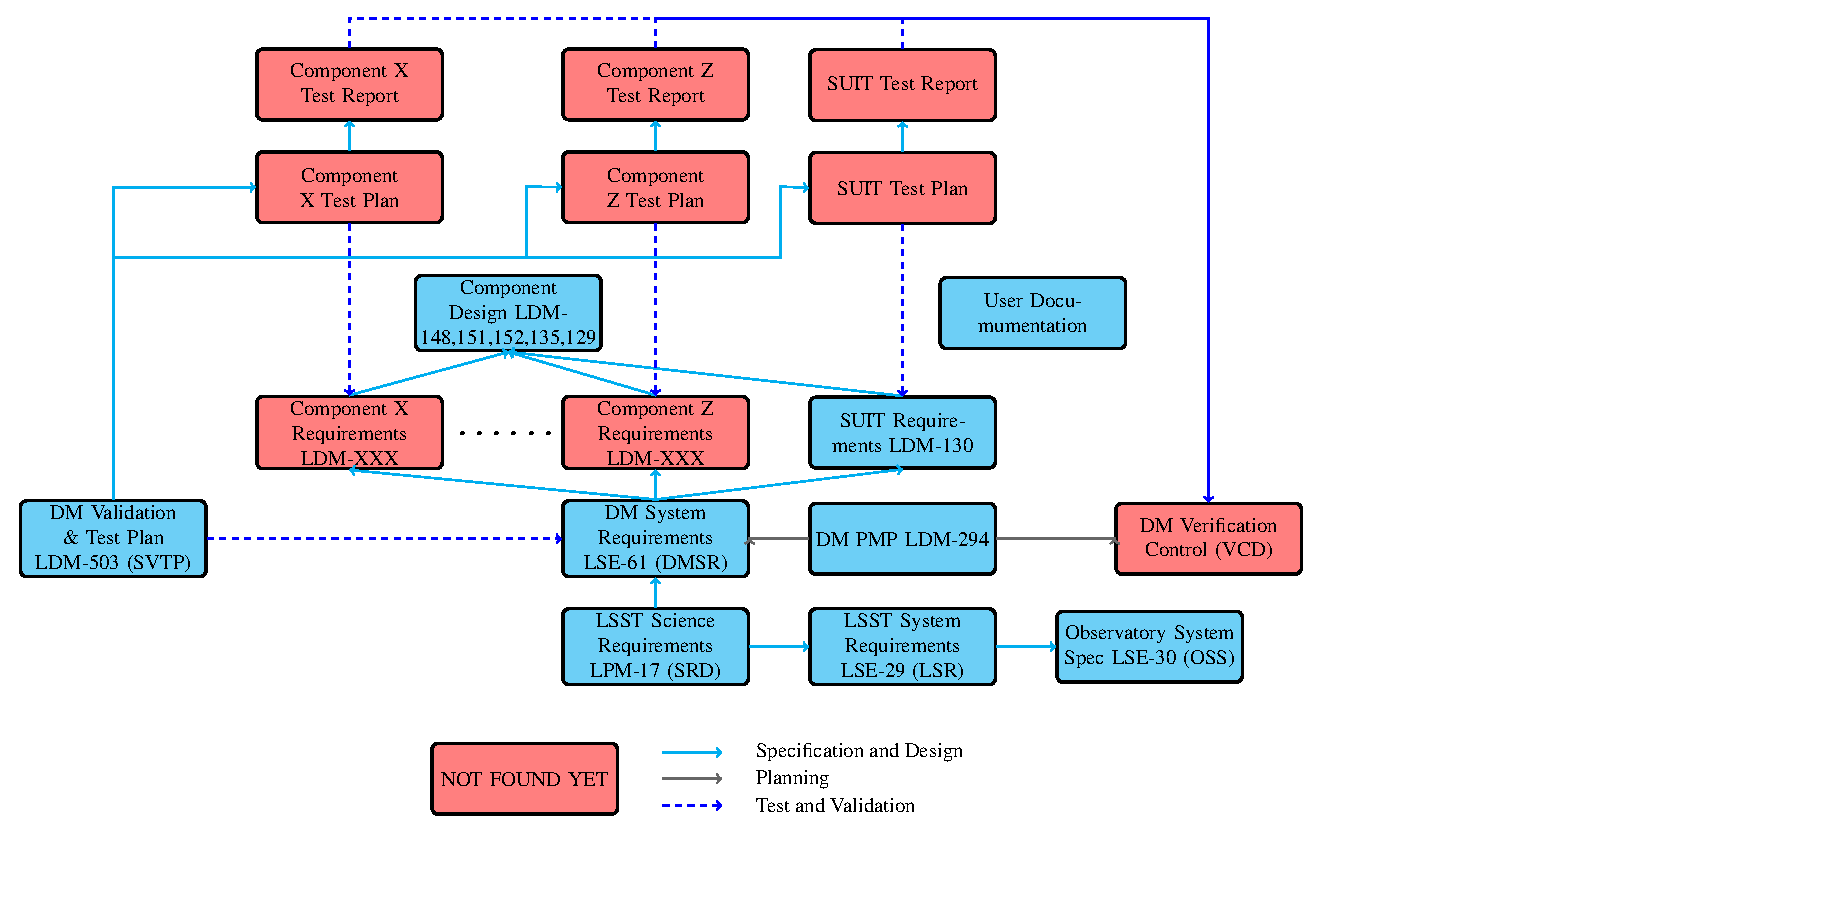
\includegraphics[width=1.2\textwidth]{images/DocTree}
\end{center}
}

\section {Milesones and Reviews }
\frame {
  \frametitle{ The re plan }
  Lots of work has gone in to the new DM plan 
\begin{center}	
   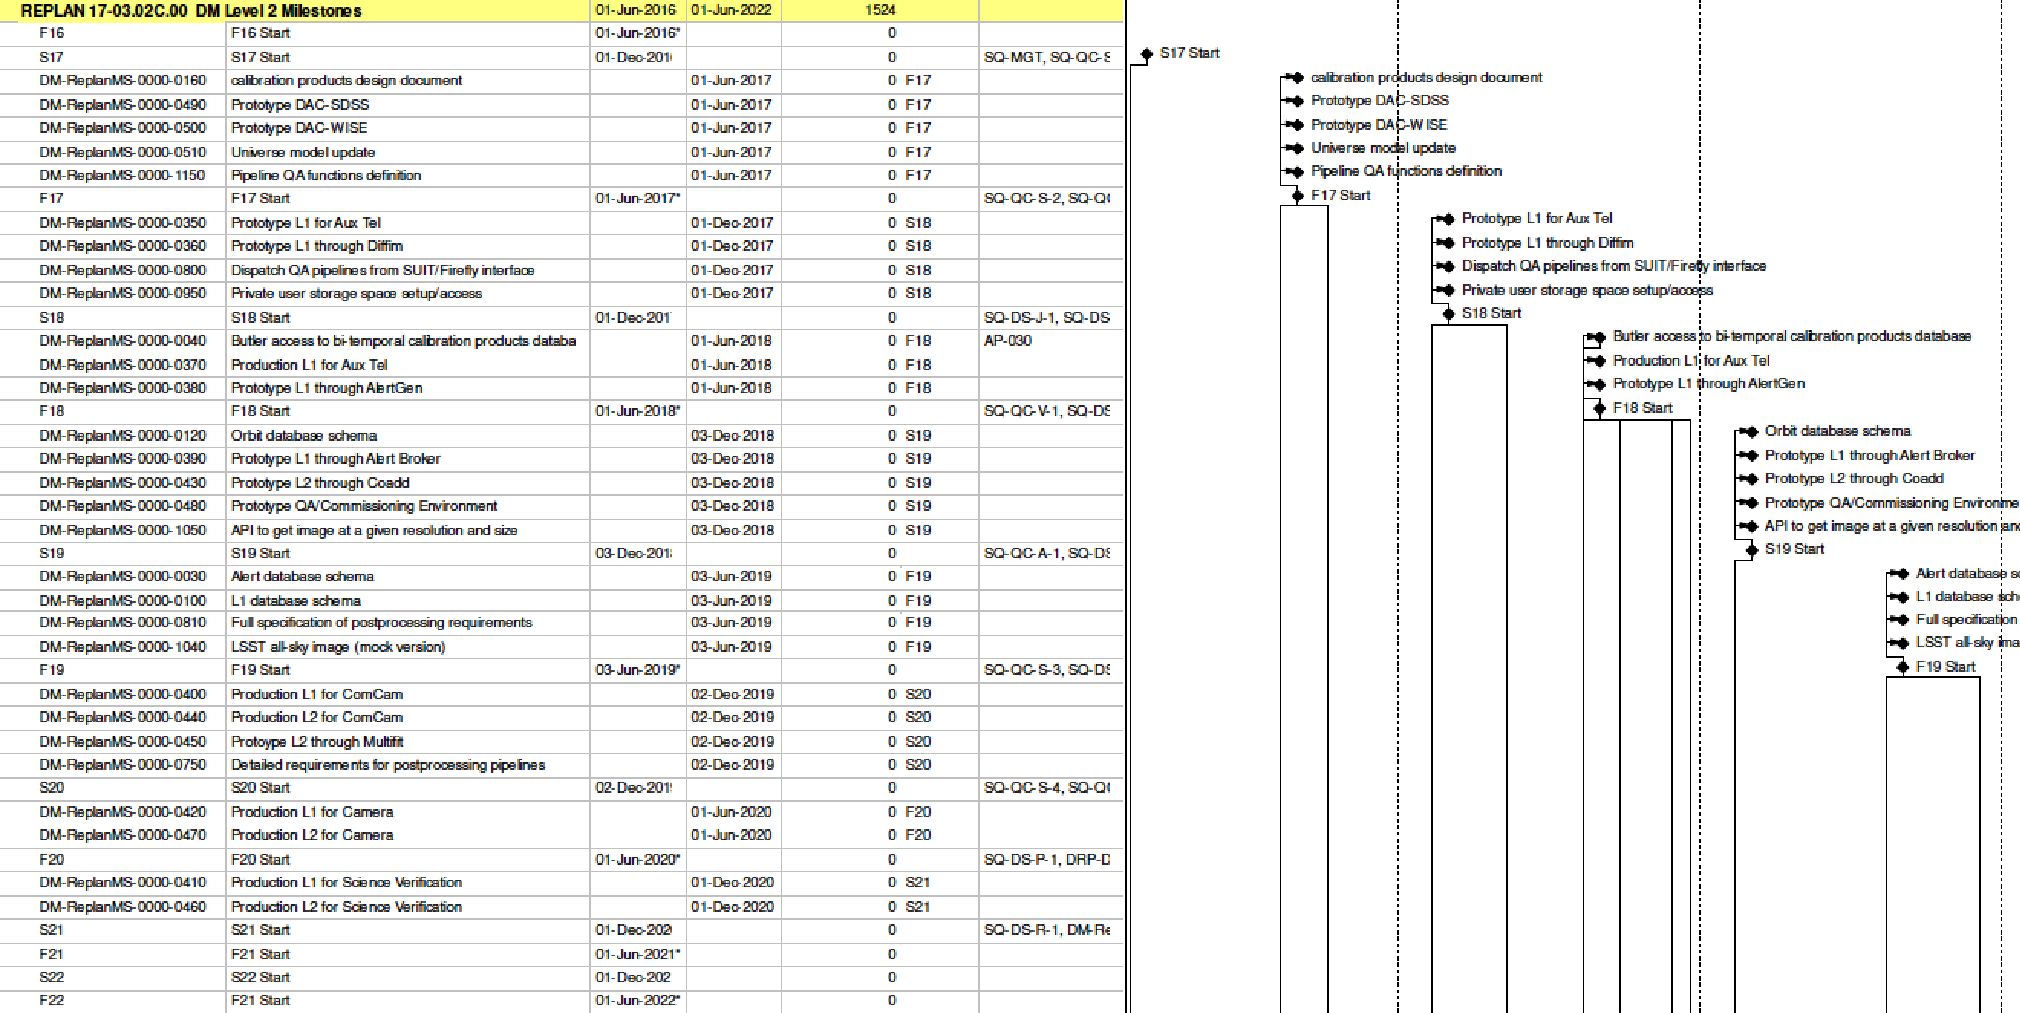
\includegraphics[width=\textwidth]{plan}
\end{center}	

}

\frame { \frametitle{ High Level Goals }
 \begin{itemize}
   \item June 2017 - Prototype Data Access Centre - with WISE Data+ 
   \item Dec 2017 - Private databases/User tables  .. Notebooks
   \item 2018 - Prototypes for various processes and databases - Minimum Viable System 
 \begin{itemize}
   \item 2018 - Mountain base network up
   \item 2018 - Prototype alerts through  broker
 \end{itemize}

   \item Dec 2019 - Com Cam L1,L2 Production
   \item Jun 2020 - Camera L1,L2 Production
   \item \ldots
 \end{itemize}
 {\em Test plans which show milestones have been met are needed.}\\
 Longer term working with Mario on which data products will come out when .. 
}

\frame{\frametitle{Reviews}
	\begin{itemize}
	\item Reviews are inevitable and necessary in large project
		\item Next DM Review {\color{red} July 25-27 }
	\item Review should confirm we are on the correct track and may indicate areas of improvement
	\item  Docs updated in each cycle – concentration before review on docs for that review. {\color{red} May be a bit more work this time}
	\item Latest released version of documents could be pulled from docushare and handed over - {\em no particular extra work iff the work is done properly anyway}
	\item Of course some presentations will be needed also ..
	\end{itemize}
}


\frame {
  \frametitle{ The END }
\begin{itemize}
\item Looking forward to working with a great set of people in DM and LSST
\item LSST has  potential for huge impact in Astronomy
\item I will use my experience and training to help get DM delivered  
\item I also have a lot to learn from LSST people so I hope you will all help me - intend to visit all the DM sites soon
\item I have an open door policy, extended to phone email in DM ! (I do close my door when in a telecon)
\item Looking forward to the first LSST images !
\end{itemize}
\begin{center}	
\huge{\color{red} Questions ??}
\end{center}	

}


\frame[allowframebreaks]{\frametitle{ Acronyms }
\vspace{10pt}
\tiny
The following table has been generated from the on-line Gaia acronym list:
\newline\newline%decrement table counter so table sin doc start at 1.
\addtocounter{table}{-1}
\begin{longtable}{|l|p{0.8\textwidth}|}\hline 
\textbf{Acronym} & \textbf{Description}  \\\hline
API&Application Programming Interface \\\hline
CU&Coordination Unit (in DPAC) \\\hline
DM&Data Management (LSST) \\\hline
DPAC&Data Processing and Analysis Consortium \\\hline
DPACE&Data Processing and Analysis Consortium Executive \\\hline
ECSS&European Cooperation for Space Standardisation \\\hline
ESA&European Space Agency \\\hline
ESAC&European Space Astronomy Centre (VilSpa) \\\hline
ESF&European Science Foundation \\\hline
ESTEC&European Space research and TEchnology Centre (ESA) \\\hline
FOP&Flight Operation Procedure (Plan) \\\hline
GIS&(Astrometric) Global Iterative Solution \\\hline
IOA&Institute of Astronomy (Cambridge; also denoted IOA) \\\hline
LDAP&Lightweight Directory Access Protocol \\\hline
LSST&Large Synoptic Surrvey Telescope \\\hline
LTD&LSST the Docs \\\hline
LaTeX&(Leslie) Lamport TeX (document markup language and document preparation system) \\\hline
MDB&Main Database \\\hline
MOC&Mission Operations Centre \\\hline
NASA&National Aeronautics and Space Administration (USA) \\\hline
PR&Progress Report \\\hline
QA&Quality Assurance \\\hline
SDSS&Sloan Digital Sky Survey \\\hline
SOC&Science Operations Centre \\\hline
SVN&SubVersioN \\\hline
TOC&Table of Contents \\\hline
USA&United States of America \\\hline
WP&Work Package \\\hline
XMM&X-ray Multi-mirror Mission (ESA; officially known as XMM-Newton) \\\hline
\end{longtable} 

}

\frame{\frametitle{ References }
\tiny
\bibliographystyle{gaia_aa}
\bibliography{lsst,gaia_livelink_valid,gaia_refs,gaia_books,gaia_refs_ads}
\normalsize

}
\end{document}
